\section{Introduction}

3D Gaussian Splatting (3DGS)~\cite{kerbl2023} reconstructs a scene from posed photographs and renders new viewpoints in real time. With many input images it is accurate; with a handful the optimisation is under-constrained, and 3DGS fits the training images with geometry that is wrong elsewhere, visible as floaters and smeared background in new views. Sparse inputs are the common case in practice: a robot that passes a place once, a quick inspection capture, or a few phone photos of an object.

A widely used remedy is to supervise the rendered depth with a pretrained monocular or multi-view depth network~\cite{dsnerf,fsgs,dngaussian}. The predicted depth is, however, least reliable exactly where guidance matters most: at depth edges, on thin structures, on sky and on textureless or reflective surfaces~\cite{indepth}. Current depth foundation models such as Depth Anything~3 (DA3)~\cite{da3} also return a per-pixel \emph{confidence}. Using it to weight the depth loss is an obvious idea, and Pi-GS~\cite{pigs} does so, but its contribution has not been measured in isolation, nor has it been checked whether the confidence actually indicates where the predicted depth is wrong.

This project asks two questions. \emph{How much does depth supervision from a current depth foundation model improve a strong sparse-view 3DGS baseline, and does weighting that supervision by the model's own confidence add anything, given how well the confidence predicts depth error?} The contributions are:
\begin{itemize}
\item A controlled study on top of DropGaussian~\cite{dropgaussian} with five loss variants that differ only in per-pixel weights, including a hard mask and a shuffled-confidence control, over multiple seeds and with paired significance tests.
\item A direct measurement of confidence calibration (sparsification curves, AUSE, AURG) and of the geometric accuracy of the trained models, both against dense reference reconstructions.
\item A new self-captured dataset, \emph{Hacettepe Statues}: \statuesnscenes{} 360$^\circ$ phone walk-arounds of outdoor sculptures, prepared with a reproducible pipeline and used as a second benchmark that nothing was tuned on.
\end{itemize}

\section{Related Work}

\textbf{Sparse-view radiance fields.} NeRF-based methods regularise few-shot reconstruction with depth from structure-from-motion~\cite{dsnerf} or with geometry and appearance priors on unseen views~\cite{regnerf}. For 3DGS, FSGS~\cite{fsgs} adds Gaussian unpooling and a Pearson-correlation loss between rendered and monocular depth; DNGaussian~\cite{dngaussian} normalises depth globally and locally before comparing it. DropGaussian~\cite{dropgaussian} uses no external prior at all: it randomly drops Gaussians during training, so that the remaining ones receive gradients and must explain the image on their own, which reduces overfitting. It is among the strongest prior-free methods and is our baseline.

\textbf{Depth priors and their reliability.} DA3~\cite{da3} predicts depth jointly from any number of views and returns a confidence map. Pi-GS~\cite{pigs} initialises 3DGS from a dense multi-view prediction and weights its depth loss by confidence. Xiao~\emph{et al.}~\cite{indepth} report that monocular depth supervision often brings little or even hurts, because the prior is wrong in the regions that matter. Whether a model's confidence ranks its own errors is usually measured with sparsification curves~\cite{ilg2018,poggi2020}: pixels are removed in order of decreasing uncertainty, and a useful uncertainty makes the remaining error fall quickly.

\section{Method}

\subsection{Baseline}
DropGaussian~\cite{dropgaussian} optimises the standard 3DGS photometric loss $\mathcal{L}_{\text{rgb}} = (1-\lambda)\,\mathcal{L}_1 + \lambda\,\mathcal{L}_{\text{D-SSIM}}$ with $\lambda = 0.2$ for 10{,}000 iterations from an initial point cloud. At iteration $t$ each Gaussian is dropped with probability $p_t = 0.2\,t/T$ and the opacity of the kept ones is scaled by $1/(1-p_t)$. We use the authors' code unmodified as a git submodule.

\subsection{Depth rendering}
Depth is rendered with a second call to the same rasteriser, in which the colour of each Gaussian is its camera-space depth $z_i$, giving $\hat D = \sum_i T_i\,\alpha_i\,z_i$; a third channel accumulates opacity. Both passes share the same DropGaussian mask and the same screen-space tensor, so the depth gradient also enters the densification statistics, as it would in a single fused rasteriser. No CUDA code is changed.

\subsection{Weighted Pearson depth loss}
Monocular and multi-view depth predictions have an unknown scale and shift, so we compare rendered depth $x = \hat D$ and prior depth $y = D_{\text{DA3}}$ by their correlation. With per-pixel weights $w$, weighted means $\bar x = \sum w x / \sum w$ (likewise $\bar y$) and
\begin{equation}
\rho_w = \frac{\sum_p w_p (x_p-\bar x)(y_p-\bar y)}{\sqrt{\sum_p w_p (x_p-\bar x)^2 \,\sum_p w_p (y_p-\bar y)^2}},
\end{equation}
the depth loss is $\mathcal{L}_d = 1 - \rho_w$ and the total loss is $\mathcal{L}_{\text{rgb}} + \lambda_d\,\mathcal{L}_d$, applied from the first iteration. With $w \equiv 1$ this is exactly the Pearson loss of FSGS. The prior and the weights are constants.

\subsection{Variants}
The five variants differ only in $w$ (Table~\ref{tab:variants}). In V2 the DA3 confidence $c$ is converted to weights by its rank within the image, $w_p = \mathrm{rank}(c_p)/(N-1)$, so the weights lie in $[0,1]$ and do not depend on the confidence scale. V3 keeps only the most confident half of the pixels. V4 is the control: it uses exactly the weights of V2 but permutes them spatially, so the amount of down-weighting is identical and only its placement is lost. If confidence carries useful information, V2 must beat V4.

\begin{table}[t]
\centering
\caption{Loss variants. All share code, initialisation, hyperparameters and seeds.}
\label{tab:variants}
\small
\begin{tabular}{@{}ll@{}}
\toprule
ID & Depth loss weights $w$ \\
\midrule
V0 & no depth loss (DropGaussian baseline) \\
V1 & uniform, $w \equiv 1$ (plain Pearson loss) \\
V2 & rank-normalised DA3 confidence (proposed) \\
V3 & 1 on the most confident 50\,\% of pixels, 0 elsewhere \\
V4 & V2's weights, spatially shuffled (control) \\
\bottomrule
\end{tabular}
\end{table}

\subsection{Depth prior}
DA3-Large (v1.1) is run once per scene, jointly on all training views (multi-view mode), at a processing resolution of 504 pixels on the long side. Depth and confidence are cached and bilinearly resized to the training resolution.

\subsection{Analysis tools}
\textbf{Reference reconstructions.} Neither benchmark has ground-truth depth. For each scene we train the baseline on \emph{all} non-test views (17--54 views for LLFF, 84 for each statue) and use its rendered depth, where its accumulated opacity exceeds 0.99, as a reference. It is a reconstruction, not ground truth, but it is far better constrained than any sparse-view model.

\textbf{Confidence calibration.} At each training view, the DA3 depth is aligned to the reference by least-squares scale and shift, and the per-pixel absolute relative error is computed. Pixels are then removed in order of increasing confidence and the mean error of the remaining ones is recorded, normalised by the full-image error. AUSE is the area between this curve and the oracle curve (removal by true error); AURG is the area between the random-removal line and the confidence curve, positive if confidence ranks errors better than chance~\cite{poggi2020}. We also report the Spearman correlation $\rho_s$ between confidence and error.

\textbf{Geometry of the trained models.} Each trained model is rendered at the held-out views and its depth (normalised by accumulated opacity) is compared with the reference depth in the same COLMAP frame, \emph{without} any alignment, by absolute relative error (AbsRel).

\section{Experimental Setup}

\subsection{LLFF}
LLFF~\cite{llff} has 8 forward-facing real scenes. We follow the standard sparse-view protocol of the baseline: images at 1/8 resolution ($504\times378$), every 8th image held out for testing, and 3 training views evenly spaced among the rest. The initial point clouds are the baseline authors' own dense clouds computed from the 3 training views, so the baseline starts from the same initialisation as in the paper.

\subsection{Hacettepe Statues}
\textbf{Capture.} On 18 November 2026 we filmed \statuesnscenes{} outdoor sculptures on the Hacettepe Beytepe campus (Fig.~\ref{fig:dataset}), one walk-around video per statue, on a Samsung Galaxy S26 Ultra held in portrait: FHD ($1080\times1920$) at 60\,fps, 1$\times$ zoom, no HDR, no flash and no motion compensation. With stabilisation off and the zoom fixed, the intrinsics stay constant within a clip. Clips are 27--56\,s long. The scenes are unbounded and 360$^\circ$, with grass, paving, trees, buildings and passers-by around the statues, and range from compact abstract stone forms to multi-figure bronze groups.

\textbf{Preparation} (\texttt{scripts/prepare\_statues.py}). Each clip is cut into 96 equal time windows and the sharpest frame of each window (variance of the Laplacian) is kept, at $720\times1280$. COLMAP~\cite{colmap} estimates poses for all 96 frames with one shared OPENCV camera, exhaustive matching and incremental mapping, and the model is undistorted to a pinhole camera ($719\times1283$). All \statuesregistered{} frames were registered, at a mean reprojection error of \statuesreproj{}\,px. The evaluation protocol mirrors the Mip-NeRF~360~\cite{mipnerf360} sparse-view setting of the baseline: every 8th frame is held out (12 test views), and 12 training views are spread evenly around the statue, about 30$^\circ$ apart. As for LLFF, the initial point cloud comes from the training views only: the model is reduced to the 12 training cameras, points are re-triangulated from their matches alone, and COLMAP PatchMatch stereo and fusion~\cite{colmapmvs} produce a dense cloud (median \statuesfused{} points). Held-out frames contribute poses for evaluation but no geometry. Training uses half resolution ($360\times642$).

\textbf{No tuning.} All hyperparameters, including $\lambda_d$, were fixed on two LLFF scenes (fern and horns) before any statue was trained, so the statues test whether the findings transfer to a different camera, scene type and view count.

\begin{figure}[t]
\centering
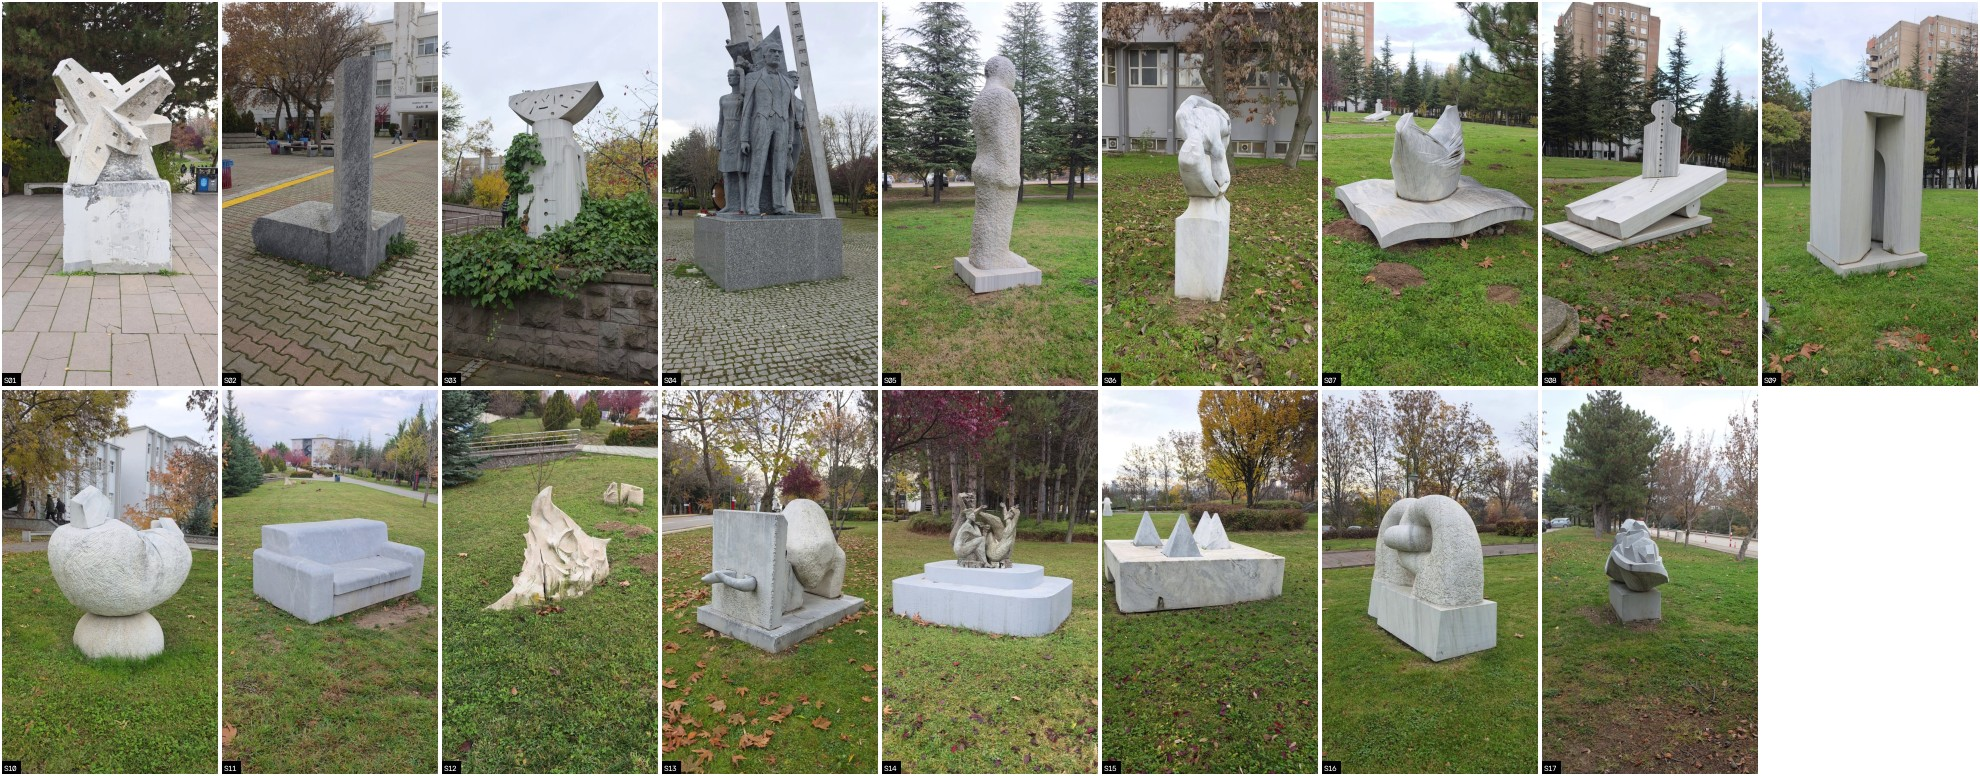
\includegraphics[width=\columnwidth]{statues_dataset.jpg}
\caption{Hacettepe Statues: the first training view of each of the \statuesnscenes{} scenes.}
\label{fig:dataset}
\end{figure}

\subsection{Implementation and protocol}
All runs use 10{,}000 iterations, $\lambda_d = 0.05$, and the baseline's other hyperparameters, on a single RTX~5060 Laptop GPU (8\,GB). Images are evaluated with the baseline's own PSNR, SSIM~\cite{ssim} and LPIPS (VGG)~\cite{lpips}. On LLFF every variant is trained with seeds 0, 1 and 2 (\LLFFnruns{} runs). On the statues, where the scene count is larger, every variant is trained with seed 0 (\Statuesnruns{} runs), because independent scenes add more statistical power than repeated seeds of the same scene. Comparisons are paired: for each scene we average the difference between two variants over seeds and apply a two-sided Wilcoxon signed-rank test~\cite{wilcoxon} to these per-scene differences. With 8 scenes, the smallest attainable $p$ is 0.008.

\section{Results}

\begin{table}[t]
\centering
\caption{Test-view image quality and held-out geometry. LLFF: mean over three seeds of the 8-scene mean, with the seed std for PSNR (for SSIM and LPIPS it is at most 0.003); Statues: seed 0, 17-scene mean. AbsRel is the rendered depth at the test views against the reference reconstruction (lower is better). Bold: best per benchmark.}
\label{tab:main}
\footnotesize
\setlength{\tabcolsep}{3.2pt}
\begin{tabular}{@{}llcccc@{}}
\toprule
 & Variant & PSNR$\uparrow$ & SSIM$\uparrow$ & LPIPS$\downarrow$ & AbsRel$\downarrow$ \\
\midrule
\multirow{5}{*}{\rotatebox{90}{LLFF}} & V0 baseline & 20.45\,$\pm$\,0.08 & 0.709 & 0.201 & 0.131 \\
 & V1 uniform & 20.91\,$\pm$\,0.07 & 0.726 & 0.189 & 0.112 \\
 & V2 confidence & 20.83\,$\pm$\,0.11 & 0.723 & 0.191 & 0.107 \\
 & V3 conf.\ half & 20.58\,$\pm$\,0.04 & 0.714 & 0.199 & 0.116 \\
 & V4 shuffled & \textbf{20.98\,$\pm$\,0.05} & \textbf{0.726} & \textbf{0.189} & 0.111 \\
\midrule
\multirow{5}{*}{\rotatebox{90}{Statues}} & V0 baseline & 17.09 & 0.438 & 0.477 & 0.315 \\
 & V1 uniform & 17.99 & 0.449 & 0.456 & 0.257 \\
 & V2 confidence & \textbf{18.21} & \textbf{0.457} & \textbf{0.449} & 0.225 \\
 & V3 conf.\ half & 17.15 & 0.443 & 0.473 & 0.275 \\
 & V4 shuffled & 18.13 & 0.452 & 0.452 & 0.242 \\
\bottomrule
\end{tabular}

\end{table}

\begin{table}[t]
\centering
\caption{Paired comparisons. $\Delta$ is the first variant minus the second, averaged per scene (over seeds on LLFF) and then over scenes. $p$: two-sided Wilcoxon signed-rank test over scenes. Wins: scenes in which the first variant has the higher PSNR.}
\label{tab:paired}
\footnotesize
\begin{tabular}{@{}llrrrrr@{}}
\toprule
 & Comparison & $\Delta$PSNR & $p$ & Wins & $\Delta$SSIM & $\Delta$AbsRel \\
\midrule
\multirow{6}{*}{\rotatebox{90}{LLFF}} & V1$-$V0 & +0.46 & 0.016 & 7/8 & +0.016 & -0.020 \\
 & V2$-$V0 & +0.38 & 0.039 & 6/8 & +0.014 & -0.024 \\
 & V2$-$V1 & -0.08 & 0.250 & 3/8 & -0.003 & -0.005 \\
 & V2$-$V4 & -0.14 & 0.008 & 0/8 & -0.003 & -0.004 \\
 & V3$-$V1 & -0.34 & 0.023 & 1/8 & -0.012 & +0.004 \\
 & V4$-$V1 & +0.06 & 0.148 & 7/8 & +0.001 & -0.001 \\
\midrule
\multirow{6}{*}{\rotatebox{90}{Statues}} & V1$-$V0 & +0.90 & <0.001 & 16/17 & +0.011 & -0.058 \\
 & V2$-$V0 & +1.11 & <0.001 & 17/17 & +0.020 & -0.090 \\
 & V2$-$V1 & +0.22 & 0.027 & 11/17 & +0.008 & -0.032 \\
 & V2$-$V4 & +0.08 & 0.174 & 12/17 & +0.005 & -0.017 \\
 & V3$-$V1 & -0.84 & <0.001 & 2/17 & -0.006 & +0.018 \\
 & V4$-$V1 & +0.14 & 0.284 & 11/17 & +0.003 & -0.015 \\
\midrule
\multirow{6}{*}{\rotatebox{90}{Both}} & V1$-$V0 & +0.76 & <0.001 & 23/25 & +0.013 & -0.046 \\
 & V2$-$V0 & +0.88 & <0.001 & 23/25 & +0.018 & -0.069 \\
 & V2$-$V1 & +0.12 & 0.141 & 14/25 & +0.005 & -0.023 \\
 & V2$-$V4 & +0.01 & 0.791 & 12/25 & +0.002 & -0.013 \\
 & V3$-$V1 & -0.68 & <0.001 & 3/25 & -0.008 & +0.013 \\
 & V4$-$V1 & +0.11 & 0.141 & 18/25 & +0.002 & -0.011 \\
\bottomrule
\end{tabular}

\end{table}

\subsection{Image quality}
Table~\ref{tab:main} gives the averages and Table~\ref{tab:paired} the paired tests.

\textbf{Depth supervision helps.} On LLFF the plain Pearson loss (V1) raises PSNR over the DropGaussian baseline by \LLFFVoneminusVzerodpsnr{}\,dB (better in \LLFFVoneminusVzerowins{} scenes, $p=\LLFFVoneminusVzerop$) and improves SSIM and LPIPS in every scene. %STATUES-V1

\textbf{Weighting by confidence does not.} The confidence-weighted loss (V2) is \LLFFVtwominusVonedpsnr{}\,dB from the plain loss on LLFF ($p=\LLFFVtwominusVonep$), and its own control, which uses the same weights at random positions (V4), is better than V2 in every LLFF scene (V2$-$V4 $=\LLFFVtwominusVfourdpsnr$\,dB, \LLFFVtwominusVfourwins{} wins, $p=\LLFFVtwominusVfourp$). Placing the low weights on the low-confidence pixels is therefore slightly \emph{harmful} for image quality compared with placing them at random. Discarding the less confident half altogether (V3) loses most of the gain of depth supervision (V3$-$V1 $=\LLFFVthreeminusVonedpsnr$\,dB, $p=\LLFFVthreeminusVonep$). %STATUES-V2

Fig.~\ref{fig:perscene} shows the per-scene gains. %STATUES-PERSCENE

\begin{figure*}[t]
\centering
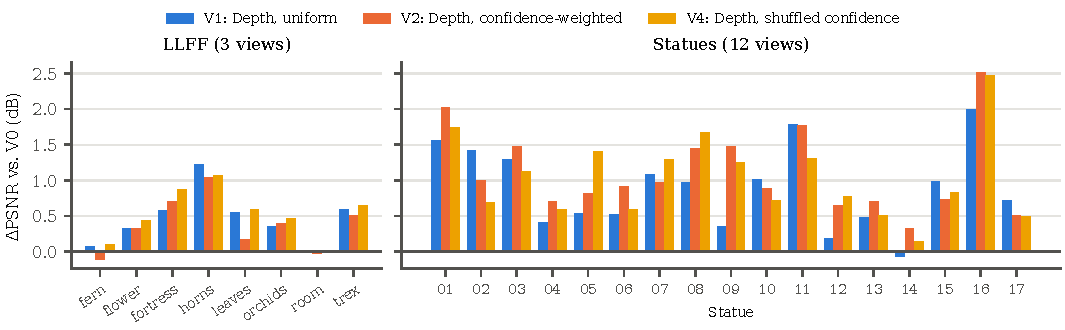
\includegraphics[width=\textwidth]{per_scene.pdf}
\caption{PSNR gain over the DropGaussian baseline per scene for the plain (V1), the confidence-weighted (V2) and the shuffled-confidence (V4) depth loss. LLFF: mean over three seeds; Statues: seed 0.}
\label{fig:perscene}
\end{figure*}

\subsection{Geometry}
Depth supervision also makes the reconstructed geometry more accurate at the held-out views (Table~\ref{tab:main}, AbsRel column): on LLFF, AbsRel falls from \LLFFVzeroabsrel{} for the baseline to \LLFFVoneabsrel{} with the plain loss (\LLFFVoneminusVzeroabsrelwins{} scenes, $p=\LLFFVoneminusVzeroabsrelp$). Here confidence weighting gives the lowest error of all variants (\LLFFVtwoabsrel{}; V2$-$V1 better in \LLFFVtwominusVoneabsrelwins{} scenes, $p=\LLFFVtwominusVoneabsrelp$), although the margin over the shuffled control is small and not significant (\LLFFVtwominusVfourabsrelwins{} scenes, $p=\LLFFVtwominusVfourabsrelp$). %STATUES-GEO
The geometry metric counts only pixels where the reference is opaque, which excludes much of the distant background; this matters for the explanation below.

\subsection{Is the confidence calibrated?}

\begin{table}[t]
\centering
\caption{Calibration of DA3 confidence against the reference depth, mean over scenes (number of scenes in brackets). AURG (depth): removing pixels farthest-first by the prior's own depth. $\rho_s(c,e)$: rank correlation of confidence and error; $|$depth: with the depth rank partialled out; $\rho_s(c,d)$: of confidence and depth.}
\label{tab:calib}
\footnotesize
\setlength{\tabcolsep}{3pt}
\begin{tabular}{@{}lcccccc@{}}
\toprule
 & AUSE$\downarrow$ & AURG$\uparrow$ & \makecell{AURG\\(depth)} & $\rho_s(c,e)$ & \makecell{$\rho_s(c,e)$\\$|$depth} & $\rho_s(c,d)$ \\
\midrule
LLFF (8) & 0.398 & 0.229 & -0.010 & -0.26 & -0.24 & -0.58 \\
Statues (17) & 0.381 & 0.261 & 0.050 & -0.24 & -0.30 & -0.84 \\
\bottomrule
\end{tabular}

\end{table}

\begin{figure}[t]
\centering
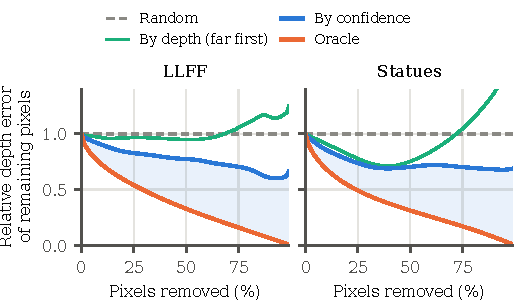
\includegraphics[width=\columnwidth]{sparsification.pdf}
\caption{Sparsification curves averaged over all training views: mean depth error of the pixels that remain when pixels are removed at random, by increasing confidence, farthest-first by predicted depth, or by decreasing true error (oracle). The shaded area is the AUSE.}
\label{fig:sparsification}
\end{figure}

Yes, partly (Table~\ref{tab:calib}, Fig.~\ref{fig:sparsification}). Removing the least confident pixels lowers the error of the rest in every LLFF scene (mean AURG \LLFFcalibaurg{}), but the confidence curve stays far from the oracle (AUSE \LLFFcalibause{}): confidence ranks errors much better than chance and much worse than perfect.

Because DA3 confidence falls with distance ($\rho_s(c,d)=\LLFFconfdepthall$ over all LLFF pixels and \Statuesconfdepthall{} over all statue pixels), a positive AURG could simply mean that far pixels are less accurate. The depth control rules this out: removing pixels farthest-first does no better than random on LLFF (AURG \LLFFcalibaurgdepth{}), confidence beats it in \LLFFcalibbeyonddepth{} scenes, and the confidence--error correlation survives partialling out depth ($\rho_s=\LLFFcalibpartial$). %STATUES-CALIB
The confidence therefore carries real information about where the prior is wrong.

\begin{figure*}[t]
\centering
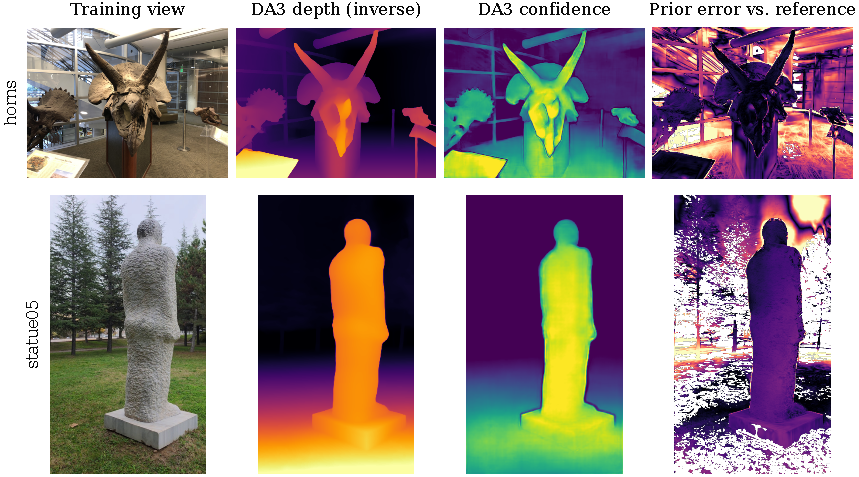
\includegraphics[width=\textwidth]{prior_error.pdf}
\caption{A training view, the DA3 depth and confidence for it, and the error of the (scale- and shift-aligned) DA3 depth against the reference, which is undefined (white) where the reference is not opaque. Low confidence covers the distant background as a whole, not only the pixels where the prior is wrong.}
\label{fig:prior}
\end{figure*}

\subsection{Why calibrated confidence does not help}
The two findings, an informative confidence and no gain from using it, are reconciled by \emph{where} the confidence-weighted loss puts its weight. Rank-normalised confidence gives the nearest third of each image (by predicted depth) a mean weight of \LLFFweightnear{} on LLFF and \Statuesweightnear{} on the statues, but the farthest third only \LLFFweightfar{} and \Statuesweightfar{} (Fig.~\ref{fig:prior}). V2 thus mostly removes depth supervision from the background, which is exactly the part of a sparse-view scene that few views constrain and where 3DGS forms floaters. The shuffled control V4 down-weights the same fraction of pixels, but uniformly over the image, so every region keeps on average half of its supervision. The ordering V3\,$<$\,V2\,$<$\,V4 in PSNR follows how much supervision reaches the background, not how accurately the remaining pixels are predicted.

Two further properties of the loss work in the same direction. First, the Pearson loss is invariant to scale and shift and compares only the shape of the depth map, so a prior that is wrong by a smooth, image-wide distortion still gives useful guidance; the errors that confidence detects are mostly local (depth edges, thin structures, sky) and matter little to a global correlation. Second, the geometry metric is restricted to pixels where the reference is opaque, which favours accurate nearby geometry; V2 is best there, while PSNR also scores the background, where V2 is weakest. For sparse-view 3DGS with a correlation loss, \emph{coverage} of the depth supervision matters more than its accuracy.

\subsection{Sensitivity to the depth weight}
%SENSITIVITY

\subsection{Qualitative results}
Fig.~\ref{fig:qualitative} shows test views from the scenes with the largest and the smallest gain of V1 over the baseline on each benchmark (\qualrows). Depth supervision mainly removes floaters and fills the background with coherent surfaces; differences between V1 and V2 are hard to see. Fly-through videos of trained models are in the repository (\texttt{demo/}).

\begin{figure*}[t]
\centering
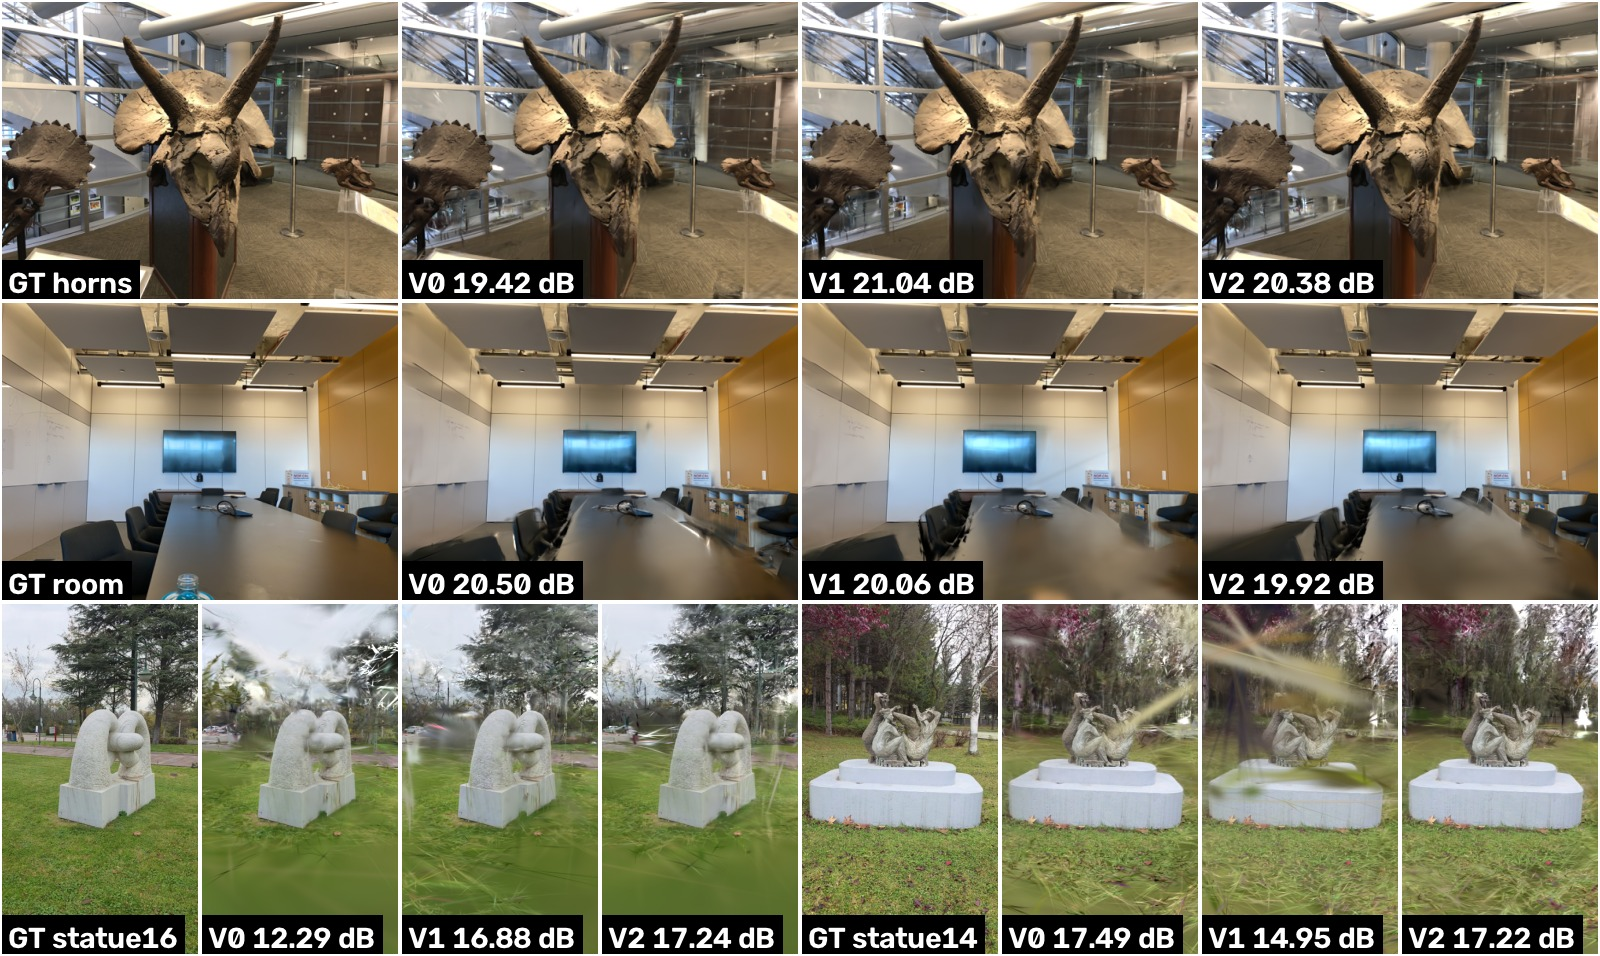
\includegraphics[width=\textwidth]{qualitative.jpg}
\caption{Test views (seed 0): ground truth, the baseline (V0), the plain depth loss (V1) and the confidence-weighted loss (V2), with per-image PSNR. Rows: \qualrows.}
\label{fig:qualitative}
\end{figure*}

\subsection{Cost}
Depth supervision needs one DA3 forward pass per scene (seconds) and a second rasterisation per iteration. The median training time rises from \LLFFVzerominutes{} to \LLFFVoneminutes{} minutes on LLFF %STATUES-COST
; the weighting itself costs nothing measurable.

\section{Discussion and Limitations}
\textbf{Reference, not ground truth.} The geometry and calibration analyses use reconstructions from all non-test views as reference. They are well constrained where views overlap but can be wrong at the image borders, on thin structures and on reflective surfaces, and they exclude non-opaque background. Errors of the reference count as errors of the prior, which would make the confidence look worse calibrated than it is, not better.

\textbf{Scope.} We test one depth model (DA3-Large), one baseline, one loss form (Pearson) and one depth weight, fixed on two LLFF scenes. The statues are trained with a single seed. Weighting schemes that keep coverage, for example normalising confidence within depth bands, or using confidence to modulate a scale-aware loss rather than a correlation, are natural next steps that our analysis suggests but does not test.

\textbf{Failure cases.} %FAILURES

\section{Conclusion}
Depth supervision from a current multi-view depth foundation model is a reliable improvement for sparse-view 3D Gaussian Splatting: it adds about half a decibel on LLFF %STATUES-CONCL
 and makes the reconstructed geometry measurably more accurate, at the price of one forward pass per scene and a second rasterisation per step. Weighting that supervision by the model's own confidence, however, does not improve image quality, even though the confidence does indicate where the predicted depth is wrong, beyond what distance alone explains. The reason is that the confidence is low over entire distant regions, and removing supervision there costs more than the errors it avoids; a shuffled-confidence control that keeps the same weights but spreads them evenly is better in every LLFF scene.

\textbf{Applications.} The pipeline turns a 30--60\,s phone video into a navigable 3D model from a dozen frames, which suits quick documentation of cultural-heritage objects such as the Hacettepe statues, site and infrastructure inspection with few passes, and robots that see a place only briefly. Our results suggest that such systems should use depth priors, and should not trust confidence-based masking to make them safer.

